
\section{Reward Hacking [5 pts]} 
Q1  illustrates how the particular  horizon and discount factor may lead to 
    to very different policies, even with the same reward and dynamics model. This may lead to unintentional reward hacking, where the resulting policy does not match a human stakeholder's intended outcome. This problem asks you to think about an example where reward hacking may occur, introduced by Pan, Bhatia and Steinhardt\footnote{ICLR 2022 \url{https://openreview.net/pdf?id=JYtwGwIL7ye}}. Consider designing RL for autonomous cars where the goal is to have decision policies that minimize the mean commute for all drivers (those driven by humans and those driven by AI). This reward might be tricky to specify (it depends on the destination of each car, etc) but a simpler reward (called the reward "proxy") is to maximize the mean velocity of all cars. Now consider a scenario where there is a single AI car (the red car in the figure) and many cars driven by humans (the grey car). 

    In this setting, under this simpler "proxy" reward, the optimal policy for the red (AI) car is to park and not merge onto the highway.\footnote{Interestingly, it turns out that systems that use simpler function representations may reward hack less in this example than more complex representations. See Pan, Bhatia and Steinhardt's paper "The Effects of Reward Misspecification: Mapping and Mitigating Misaligned Models" for details.}
        \begin{figure}[h]
    \centering
    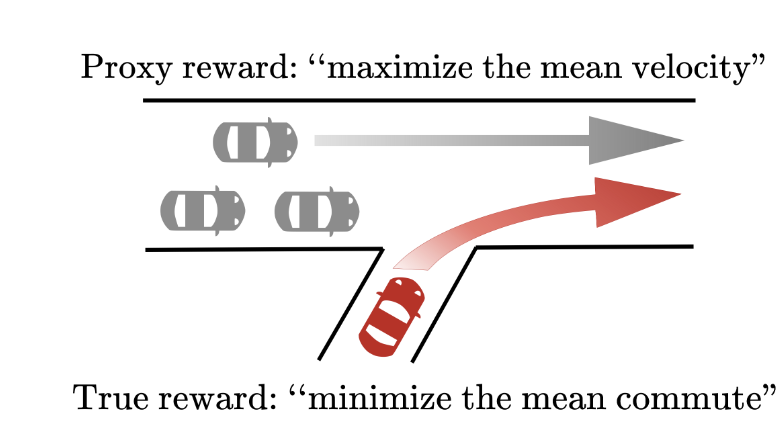
\includegraphics[width=3in]{commute_time.png}
    \caption{Pan, Bhatia, Steinhardt ICLR 2022; \url{https://openreview.net/pdf?id=JYtwGwIL7ye}}
    \label{fig:commute}
\end{figure}
\begin{enumerate}[label=(\alph*)]
    \item  Explain why the optimal policy for the AI car is not to merge onto the highway. [2 pts]
    \item Note this behavior is not aligned with the true reward function. Share some ideas about alternate reward functions (that are not minimizing commute) that might still be easier to optimize, but would not result in the AI car never merging. Your answer should be 2-5 sentences and can include equations: there is not a single answer and reasonable solutions will be given full credit. [3 pts]

\end{enumerate}

